\documentclass[11pt]{amsart}
\usepackage[margin=1.15in]{geometry}
\usepackage[T1]{fontenc}
\usepackage{lmodern}
\usepackage{amssymb,amsmath,mathtools}
\usepackage{graphicx,float}
\usepackage[hidelinks]{hyperref}
\usepackage[expansion=false]{microtype}

\newtheorem{theorem}{Theorem}[section]
\newtheorem{proposition}[theorem]{Proposition}
\newtheorem{lemma}[theorem]{Lemma}
\newtheorem{corollary}[theorem]{Corollary}
\newtheorem{mainthm}{Theorem}
\renewcommand{\themainthm}{\Alph{mainthm}}
\theoremstyle{definition}
\newtheorem{definition}[theorem]{Definition}
\newtheorem{remark}[theorem]{Remark}

\newcommand{\RR}{\mathbb{R}}
\newcommand{\Sph}{\mathbb{S}}
\newcommand{\dd}{\,\mathrm{d}}
\newcommand{\jb}[1]{\langle #1\rangle}
\newcommand{\nb}{\|b\|}

\setlength{\emergencystretch}{2.5em}
\hbadness=2000
\raggedbottom
\begin{document}

\title[Wasserstein distance along the Boltzmann flow]{The Wasserstein Distance Between Two\\ Boltzmann Solutions Can Increase}

\author{Deep Bhattacharjee}
\address{Formerly, Electro-Gravitational Space Propulsion Laboratory (EGSPL), Bhubaneswar, Odisha 751030, India}
\address{Formerly, University of Calcutta (Heramba Chandra College), 23/49 Gariahat Road, Golpark, Kolkata 700029, West Bengal, India}
\email{d.bhattacharjee@erl-forschung.de}
\email{itsdeep@live.com}
\email{egspl@proton.me (GitHub-related contact; GitHub account creelie)}
\urladdr{https://orcid.org/0000-0003-0466-750X}

\begin{abstract}
For Maxwell molecules, Tanaka proved that the quadratic Wasserstein distance between two solutions of the spatially homogeneous Boltzmann equation never increases. Villani asked whether this remains true for other collision kernels. We show that it does not: for every hard potential with angular cutoff, hard spheres included, there are smooth initial data for which the distance strictly increases. The proof is analytic and rests on an explicit Kantorovich dual certificate.

\medskip\noindent\textbf{Keywords:} Boltzmann equation; Wasserstein distance; hard potentials.

\smallskip\noindent\textbf{MSC 2020:} 35Q20 (primary); 82C40, 49Q22.
\end{abstract}

\maketitle

\section{Introduction}\label{sec:intro}

The spatially homogeneous Boltzmann equation
\begin{equation}\label{eq:B}
\partial_t f=Q(f,f),\qquad Q(f,f)(v)=\int_{\RR^3}\int_{\Sph^2}B(v-v_*,\sigma)\big(f(v')f(v'_*)-f(v)f(v_*)\big)\dd\sigma\dd v_*,
\end{equation}
with post-collisional velocities
\begin{equation}\label{eq:sigma}
v'=\frac{v+v_*}{2}+\frac{|v-v_*|}{2}\,\sigma,\qquad v'_*=\frac{v+v_*}{2}-\frac{|v-v_*|}{2}\,\sigma,
\end{equation}
describes a spatially uniform rarefied gas whose velocity distribution is $f(t,v)$. Collisions conserve mass, momentum and kinetic energy, and the entropy $\int f\log f$ decreases. We take kernels of the form
\begin{equation}\label{eq:kernel}
B(z,\sigma)=|z|^\gamma\, b(k\cdot\sigma),\qquad k=\frac{z}{|z|},\qquad 0<\gamma\le 2,
\end{equation}
with $b\ge0$ continuous on $(-1,1)$, not identically zero, and satisfying Grad's cutoff condition
\begin{equation}\label{eq:cutoff}
\nb:=\int_{\Sph^2}b(k\cdot\sigma)\dd\sigma=2\pi\int_{-1}^{1}b(x)\dd x<\infty .
\end{equation}
These are the hard potentials with angular cutoff. Hard spheres correspond to $\gamma=1$ and constant $b$. Maxwell molecules correspond to $\gamma=0$.

For two probability measures $\mu,\nu$ on $\RR^3$ with finite second moments let
\[
W_2(\mu,\nu)^2=\inf_{\pi}\iint|x-y|^2\dd\pi(x,y),
\]
the infimum running over couplings of $\mu$ and $\nu$. Tanaka discovered that for Maxwell molecules the map $t\mapsto W_2(f_t,g_t)$ is nonincreasing whenever $f$ and $g$ are two solutions of \eqref{eq:B} \cite{Tan73,Tan78}; Toscani and Villani turned related Fourier and Wasserstein metrics into a uniqueness theory for Maxwell gases \cite{TV99}. Tanaka's proof couples the collision histories of the two gases. This works because for Maxwell molecules the collision rate does not depend on the relative speed, so collisions in the two gases can be synchronised.

For other kernels only weaker statements are available, namely stability estimates in which $W_2$ or related distances may grow by a multiplicative factor. In his recent memoir on Fisher information, after the proof with Imbert and Silvestre that the Fisher information decreases along \eqref{eq:B} for all physically relevant kernels \cite{ISV25}, extending the Landau theorem of Guillen and Silvestre \cite{GS25}, Villani asked in the concluding section of \cite{Vil25} whether the same robustness holds for $W_2$: various authors have shown that this distance is exponentially stable along the Boltzmann flow for various kernels, but could it actually be nonincreasing? For the Landau equation with Maxwellian molecules contractivity holds, and for soft potentials a conditional exponential stability estimate is known \cite{CDGT25}; in the setting of granular media Carrillo, McCann and Villani proved contraction in $W_2$ for uniformly convex interactions \cite{CMV05}.

We answer the question in the negative for hard potentials. Fix the unit vector $e=(0,0,1)$ and a nonnegative even function $\eta\in C_c^\infty(\RR^3)$ with $\int\eta=1$ and support in the closed unit ball. For $0<\delta\le1$ and $\rho>0$ set $\eta_\delta(v)=\delta^{-3}\eta(v/\delta)$ and
\begin{equation}\label{eq:data}
j^\delta_\rho(v)=\tfrac12\big(\eta_\delta(v-\rho e)+\eta_\delta(v+\rho e)\big).
\end{equation}
This is a smooth probability density with zero momentum: two opposite jets of speed $\rho$, each of width $\delta$. Define
\begin{equation}\label{eq:J}
J=\int_{\Sph^2}b(e\cdot\sigma)\,\min\{1,\,s|\sigma-e|,\,s|\sigma+e|\}\dd\sigma ,
\qquad
\Gamma=\frac{2^{\gamma-1}\,(r^\gamma-s^\gamma)^2\,J^2}{s\,r^{\gamma-1}\,\nb}.
\end{equation}
Since $b$ is not identically zero and the integrand of $J$ vanishes only at $\sigma=\pm e$, we have $J>0$; hence $\Gamma>0$ whenever $r\neq s$ and $\gamma\ne0$.

\begin{mainthm}\label{thm:A}
Let $B$ satisfy \eqref{eq:kernel}--\eqref{eq:cutoff}, let $0<s<r$, and let $f^\delta$ and $g^\delta$ be the solutions of \eqref{eq:B} with initial data $j^\delta_r$ and $j^\delta_s$. There is $t_1>0$ with the following property. For every $t\in(0,t_1]$ there is $\delta_1(t)>0$ such that for all $\delta\in(0,\delta_1(t)]$
\[
W_2\big(f^\delta_t,g^\delta_t\big)^2\ \ge\ W_2\big(f^\delta_0,g^\delta_0\big)^2+\frac{\Gamma}{8}\,t .
\]
\end{mainthm}

\begin{corollary}\label{cor:no}
For every kernel \eqref{eq:kernel}--\eqref{eq:cutoff}, and in particular for hard spheres, there exist two smooth, compactly supported initial data with the same mass and momentum whose solutions satisfy $W_2(f_t,g_t)>W_2(f_0,g_0)$ for some $t>0$. Thus $t\mapsto W_2(f_t,g_t)$ is not nonincreasing.
\end{corollary}

The mechanism is simple. A pair of opposite jets of speed $\rho$ collides head-on, at relative speed $2\rho$, and every such collision sends the two particles to a pair of opposite points $\pm\rho\sigma$ of the sphere of radius $\rho$. The two gases therefore have the same geometry, only scaled, but the faster one loses its jets at the rate $(2r)^\gamma\nb/2$ and the slower one at the rate $(2s)^\gamma\nb/2$ (Figure~\ref{fig:jets}). At time zero the optimal transport between the gases is the dilation $x\mapsto(s/r)x$. After a short time the faster gas has spread more of its mass over its sphere than the slower gas has over its own, and part of this surplus must be carried back to the poles of the smaller sphere. For Maxwell molecules the two rates coincide, the dilation stays optimal, and Tanaka's theorem is recovered in this example.

\begin{figure}[H]
\centering
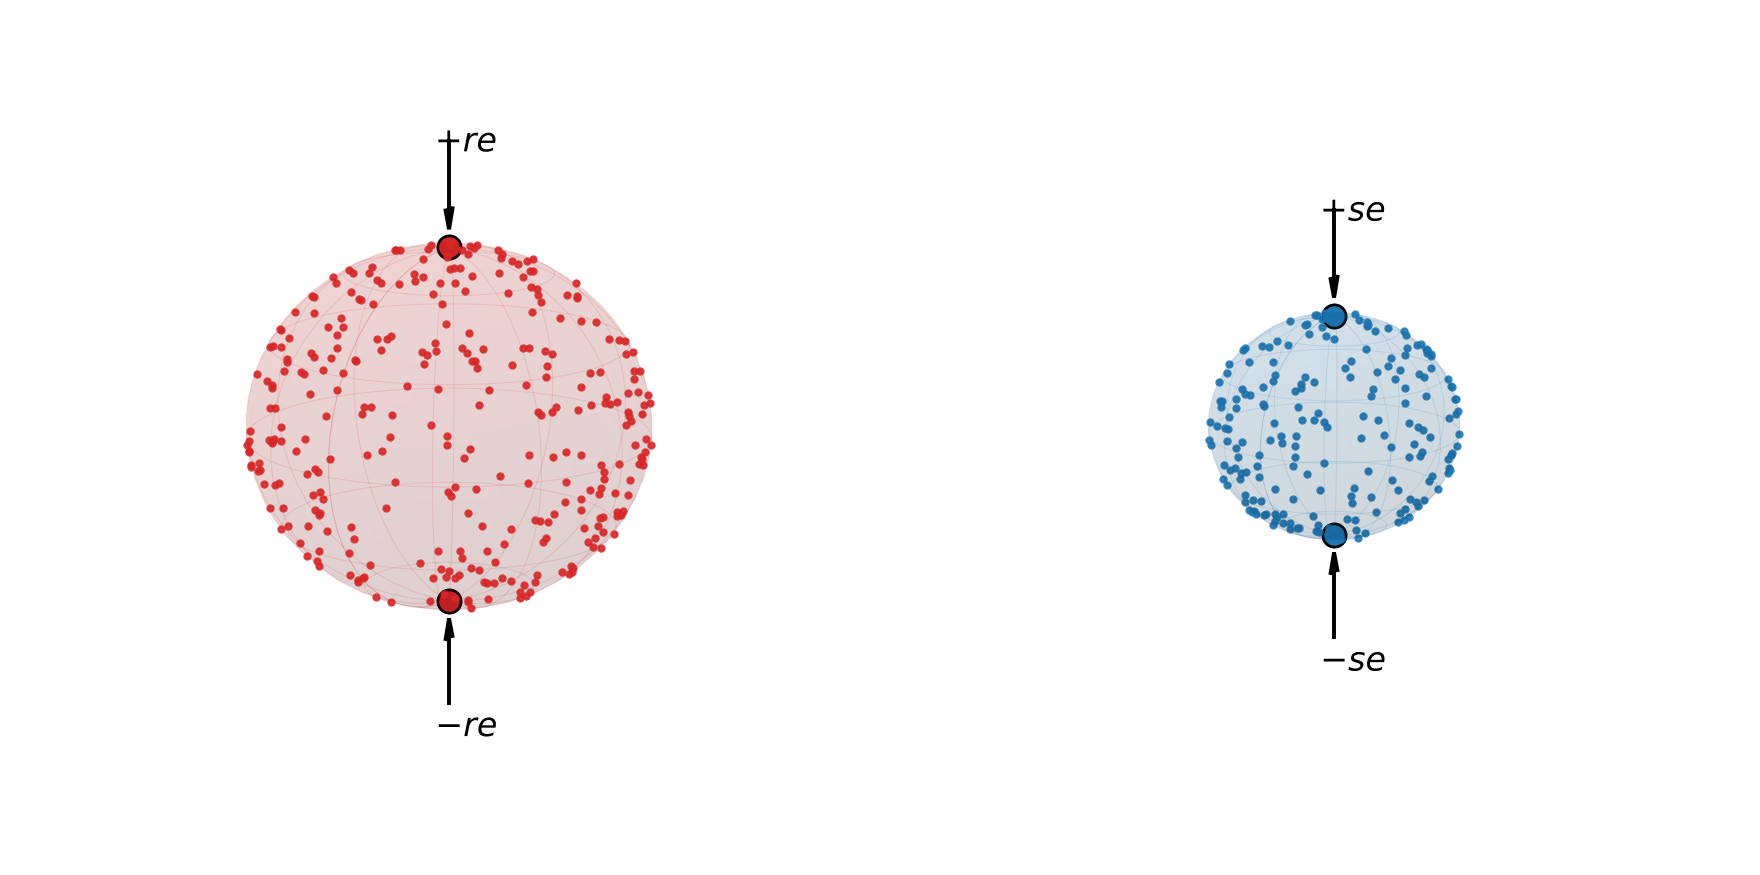
\includegraphics[width=0.9\textwidth]{fig_jets.png}
\caption{The two gases of Theorem~\ref{thm:A} shortly after time zero. Head-on collisions move mass from the jets $\pm re$ and $\pm se$ to the spheres of radii $r$ and $s$, at rates proportional to $r^\gamma$ and $s^\gamma$. The dots indicate the mass that has left the jets.}\label{fig:jets}
\end{figure}

The statement is made quantitative by Kantorovich duality, used only in its elementary direction: any pair of functions $\varphi,\psi$ with $\varphi(x)+\psi(y)\le|x-y|^2$ gives the lower bound $W_2(\mu,\nu)^2\ge\int\varphi\dd\mu+\int\psi\dd\nu$. We build such a pair from the dilation potentials by a small perturbation that rewards mass on the smaller sphere for staying at its poles (Section~\ref{sec:dual}). Its first variation along the flow is computed exactly in the limit of thin jets (Section~\ref{sec:dirac}), and a short-time expansion with uniform moment bounds controls the error (Section~\ref{sec:expansion}).

\section{Weak form and moments}\label{sec:weak}

Write $\jb{v}=(1+|v|^2)^{1/2}$ and $M_k(f)=\int\jb{v}^kf\dd v$. For a bounded continuous function $\varphi$ on $\RR^3$ define, for $v\ne v_*$,
\begin{equation}\label{eq:L}
L_\varphi(v,v_*)=|v-v_*|^\gamma\int_{\Sph^2}b(k\cdot\sigma)\big(\varphi(v')+\varphi(v'_*)-\varphi(v)-\varphi(v_*)\big)\dd\sigma,\qquad k=\frac{v-v_*}{|v-v_*|},
\end{equation}
and $L_\varphi(v,v)=0$. For a finite nonnegative measure $\mu$ with $M_\gamma(\mu)<\infty$ put
\begin{equation}\label{eq:Lambda}
\Lambda_\varphi(\mu)=\frac12\iint L_\varphi(v,v_*)\dd\mu(v)\dd\mu(v_*).
\end{equation}
When $\mu=f\dd v$ with $M_{2\gamma}(f)<\infty$, the change of variables $(v,v_*,\sigma)\mapsto(v',v'_*,k)$, which has unit Jacobian and preserves $B$, gives the classical weak form $\int\varphi\,Q(f,f)\dd v=\Lambda_\varphi(f)$; see \cite[Chap.~1]{Vil02}.

\begin{lemma}\label{lem:cont}
For bounded continuous $\varphi$, the function $L_\varphi$ is continuous on $\RR^3\times\RR^3$ and $|L_\varphi(v,v_*)|\le4\|\varphi\|_\infty\nb\,|v-v_*|^\gamma\le 4\|\varphi\|_\infty\nb\,\jb{v}^\gamma\jb{v_*}^\gamma$.
\end{lemma}

\begin{proof}
The bracket in \eqref{eq:L} is at most $4\|\varphi\|_\infty$, which gives the first bound. The second follows from $|v-v_*|\le|v|+|v_*|\le\jb{v}\jb{v_*}$, the last step being $2|v||v_*|\le1+|v|^2|v_*|^2$. The first bound shows that $L_\varphi$ is continuous on the diagonal, where it vanishes, because $\gamma>0$. Let $(v_n,v_{*n})\to(v,v_*)$ with $v\ne v_*$, and let $k_n,k$ be the corresponding unit vectors. Choose rotations $R_n\to I$ with $R_nk=k_n$. The substitution $\sigma=R_n\omega$ turns the integral in \eqref{eq:L} at $(v_n,v_{*n})$ into $\int b(k\cdot\omega)\Psi_n(R_n\omega)\dd\omega$, where $\Psi_n(\sigma)$ is the bracket evaluated at $(v_n,v_{*n},\sigma)$. These functions are bounded by $4\|\varphi\|_\infty$ and converge pointwise to the bracket at $(v,v_*,\omega)$, by \eqref{eq:sigma} and the continuity of $\varphi$. Since $b(k\cdot\omega)$ is integrable, dominated convergence gives continuity at $(v,v_*)$.
\end{proof}

We use the $L^1$ theory of \eqref{eq:B} for hard potentials with cutoff, due to Arkeryd, Elmroth, Desvillettes, Wennberg, and Mischler and Wennberg \cite{MW99,Wen97}. For every nonnegative $f_0$ with $M_2(f_0)<\infty$ there is a unique solution $f\in C([0,\infty);L^1_2)$ that conserves mass, momentum and energy and satisfies $f_t=f_0+\int_0^tQ(f_\tau,f_\tau)\dd\tau$; moreover, every moment that is finite at time zero stays bounded in time \cite[Sect.~1]{MW99}, \cite{Wen97}. Our data \eqref{eq:data} have compact support, so all their moments are finite and the moment identities below are justified.

\begin{lemma}\label{lem:moments}
Let $K_0\ge M_4(f_0)$ and $T=(2\nb K_0)^{-1}$. Then $M_4(f_t)\le 2K_0$ for $0\le t\le T$.
\end{lemma}

\begin{proof}
Applying the weak form to $\varphi=\jb{v}^4$ (legitimate because $M_6$ is locally bounded),
\[
\frac{\dd}{\dd t}M_4(f_t)=\frac12\iint f f_*|v-v_*|^\gamma\int b(k\cdot\sigma)\big(\jb{v'}^4+\jb{v'_*}^4-\jb{v}^4-\jb{v_*}^4\big)\dd\sigma\dd v\dd v_* .
\]
Energy conservation gives $\jb{v'}^2+\jb{v'_*}^2=\jb{v}^2+\jb{v_*}^2$, so $\jb{v'}^4+\jb{v'_*}^4\le(\jb{v}^2+\jb{v_*}^2)^2$ and the bracket is at most $2\jb{v}^2\jb{v_*}^2$. With $|v-v_*|^\gamma\le\jb{v}^\gamma\jb{v_*}^\gamma$ and $\gamma\le2$ we get $\frac{\dd}{\dd t}M_4\le\nb M_{2+\gamma}^2\le\nb M_4^2$. Hence $M_4(f_t)\le K_0/(1-\nb K_0t)\le2K_0$ for $t\le T$.
\end{proof}

\section{A short-time expansion}\label{sec:expansion}

\begin{lemma}\label{lem:expansion}
Let $f$ be a solution with $M_4(f_\tau)\le K$ for $0\le\tau\le t$. Then for every bounded continuous $\varphi$
\[
\Big|\int\varphi f_t-\int\varphi f_0-t\,\Lambda_\varphi(f_0)\Big|\le 8\,\|\varphi\|_\infty\nb^2K^3\,t^2 .
\]
\end{lemma}

\begin{proof}
First, $\|Q(f,f)\|_{L^1_\gamma}\le4\nb M_{2\gamma}(f)M_\gamma(f)$. Indeed $\int\jb{v}^\gamma|Q(f,f)|\le\iiint Bff_*(\jb{v'}^\gamma+\jb{v}^\gamma)$, by the same change of variables applied to the gain term, and $\jb{v'}^\gamma\le(\jb{v}^2+\jb{v_*}^2)^{\gamma/2}\le\jb{v}^\gamma+\jb{v_*}^\gamma$ because $\gamma\le2$; together with $|v-v_*|^\gamma\le\jb{v}^\gamma\jb{v_*}^\gamma$ the integrand is at most $2\nb ff_*\jb{v}^\gamma\jb{v_*}^\gamma(\jb{v}^\gamma+\jb{v_*}^\gamma)$ after integration in $\sigma$. Since $M_\gamma\le M_{2\gamma}\le M_4$, the identity $f_\tau-f_0=\int_0^\tau Q(f_u,f_u)\dd u$ gives $\|f_\tau-f_0\|_{L^1_\gamma}\le4\nb K^2\tau$.

Next, by Lemma~\ref{lem:cont} and $|f_\tau f_{\tau*}-f_0f_{0*}|\le|f_\tau-f_0|f_{\tau*}+f_0|f_{\tau*}-f_{0*}|$,
\[
|\Lambda_\varphi(f_\tau)-\Lambda_\varphi(f_0)|\le 2\|\varphi\|_\infty\nb\,\|f_\tau-f_0\|_{L^1_\gamma}\big(M_\gamma(f_\tau)+M_\gamma(f_0)\big)\le16\,\|\varphi\|_\infty\nb^2K^3\,\tau .
\]
Finally $\int\varphi f_t-\int\varphi f_0=\int_0^t\Lambda_\varphi(f_\tau)\dd\tau$, and integrating the last bound over $[0,t]$ proves the lemma.
\end{proof}

\section{The dual certificate}\label{sec:dual}

Let $0<s<r$. The dilation $x\mapsto(s/r)x$ is the gradient of a convex function, and the corresponding Kantorovich potentials for the cost $|x-y|^2$ are $\varphi_0(x)=(1-\frac sr)|x|^2$ and $\psi_0(y)=(1-\frac rs)|y|^2$. Indeed, completing the square,
\begin{equation}\label{eq:square}
|x-y|^2-\psi_0(y)=\frac rs\Big|y-\frac srx\Big|^2+\varphi_0(x).
\end{equation}
Set
\[
h(y)=\min\{1,\,|y-se|,\,|y+se|\},
\]
a $1$-Lipschitz even function with values in $[0,1]$ which vanishes exactly at $\pm se$. For $\varepsilon>0$ define
\begin{equation}\label{eq:pair}
\psi_\varepsilon=\psi_0-\varepsilon h,\qquad
\varphi_\varepsilon(x)=\inf_{y\in\RR^3}\big(|x-y|^2-\psi_\varepsilon(y)\big).
\end{equation}
By construction $\varphi_\varepsilon(x)+\psi_\varepsilon(y)\le|x-y|^2$ for all $x,y$. By \eqref{eq:square},
\begin{equation}\label{eq:phieps}
\varphi_\varepsilon(x)=\varphi_0(x)+m_\varepsilon\Big(\frac srx\Big),\qquad m_\varepsilon(z)=\inf_{y\in\RR^3}\Big(\frac rs|y-z|^2+\varepsilon h(y)\Big).
\end{equation}

\begin{lemma}\label{lem:m}
The function $m_\varepsilon$ is even and continuous, $0\le m_\varepsilon\le\varepsilon h\le\varepsilon$, $m_\varepsilon(\pm se)=0$, and
\[
m_\varepsilon(z)\ge\varepsilon h(z)-\frac{s\,\varepsilon^2}{4r}\qquad(z\in\RR^3).
\]
\end{lemma}

\begin{proof}
Evenness follows from that of $h$, and the upper bound from the choice $y=z$. The infimum may be restricted to $|y-z|\le(s\varepsilon/r)^{1/2}$, where the functions $z\mapsto\frac rs|y-z|^2$ are uniformly Lipschitz, so $m_\varepsilon$ is locally Lipschitz. Since $h$ is $1$-Lipschitz, $\frac rs|y-z|^2+\varepsilon h(y)\ge\varepsilon h(z)+\frac rsu^2-\varepsilon u$ with $u=|y-z|$, and $\min_{u\ge0}(\frac rsu^2-\varepsilon u)=-s\varepsilon^2/(4r)$.
\end{proof}

So $\varphi_\varepsilon$ and $\psi_\varepsilon$ split into the energy terms $\varphi_0,\psi_0$ and the bounded continuous parts
\begin{equation}\label{eq:tilde}
\tilde\varphi_\varepsilon(x)=m_\varepsilon\Big(\frac srx\Big),\qquad\tilde\psi_\varepsilon=-\varepsilon h,\qquad \|\tilde\varphi_\varepsilon\|_\infty,\ \|\tilde\psi_\varepsilon\|_\infty\le\varepsilon .
\end{equation}

\section{The thin-jet limit}\label{sec:dirac}

Let $P_\rho=\frac12(\delta_{\rho e}+\delta_{-\rho e})$, the weak limit of $j^\delta_\rho$ as $\delta\to0$.

\begin{lemma}\label{lem:dirac}
For every even bounded continuous $\varphi$,
\[
\Lambda_\varphi(P_\rho)=2^{\gamma-1}\rho^\gamma\int_{\Sph^2}b(e\cdot\sigma)\big(\varphi(\rho\sigma)-\varphi(\rho e)\big)\dd\sigma .
\]
\end{lemma}

\begin{proof}
By \eqref{eq:Lambda}, $\Lambda_\varphi(P_\rho)=\frac18\big(L_\varphi(\rho e,\rho e)+L_\varphi(-\rho e,-\rho e)+L_\varphi(\rho e,-\rho e)+L_\varphi(-\rho e,\rho e)\big)$. The first two terms vanish. For $(v,v_*)=(\rho e,-\rho e)$ we have $k=e$, $v'=\rho\sigma$, $v'_*=-\rho\sigma$, and for $(v,v_*)=(-\rho e,\rho e)$ we have $k=-e$ and the same $v',v'_*$. The substitution $\sigma\mapsto-\sigma$ shows that the two cross terms are equal, so
\[
\Lambda_\varphi(P_\rho)=\frac14(2\rho)^\gamma\int b(e\cdot\sigma)\big(\varphi(\rho\sigma)+\varphi(-\rho\sigma)-\varphi(\rho e)-\varphi(-\rho e)\big)\dd\sigma,
\]
and evenness of $\varphi$ gives the claim.
\end{proof}

\begin{proposition}\label{prop:gain}
With $\tilde\varphi_\varepsilon,\tilde\psi_\varepsilon$ as in \eqref{eq:tilde} and $J$ as in \eqref{eq:J},
\[
\Gamma_\varepsilon:=\Lambda_{\tilde\varphi_\varepsilon}(P_r)+\Lambda_{\tilde\psi_\varepsilon}(P_s)\ \ge\ 2^{\gamma-1}\Big(\varepsilon\,(r^\gamma-s^\gamma)\,J-\frac{\varepsilon^2}{4}\,s\,r^{\gamma-1}\nb\Big).
\]
For $\varepsilon_*=2(r^\gamma-s^\gamma)J/(s\,r^{\gamma-1}\nb)$ the right-hand side equals the number $\Gamma$ of \eqref{eq:J}.
\end{proposition}

\begin{proof}
Both functions are even. On the sphere of radius $r$ we have $\tilde\varphi_\varepsilon(r\sigma)=m_\varepsilon(s\sigma)$ and $\tilde\varphi_\varepsilon(re)=m_\varepsilon(se)=0$; on the sphere of radius $s$, $\tilde\psi_\varepsilon(s\sigma)=-\varepsilon h(s\sigma)$ and $\tilde\psi_\varepsilon(se)=0$. Note that $h(s\sigma)=\min\{1,s|\sigma-e|,s|\sigma+e|\}$. Lemma~\ref{lem:dirac} therefore gives
\[
\Gamma_\varepsilon=2^{\gamma-1}\Big(r^\gamma\int b(e\cdot\sigma)\,m_\varepsilon(s\sigma)\dd\sigma-\varepsilon s^\gamma J\Big).
\]
By Lemma~\ref{lem:m}, $\int b(e\cdot\sigma)m_\varepsilon(s\sigma)\dd\sigma\ge\varepsilon J-s\varepsilon^2\nb/(4r)$, which yields the inequality. The value at $\varepsilon_*$ is a direct computation.
\end{proof}

\section{Proof of Theorem~\ref{thm:A}}\label{sec:proof}

Fix $\varepsilon=\varepsilon_*$, so that $\Gamma_\varepsilon\ge\Gamma>0$. All the data $j^\delta_r$, $j^\delta_s$ with $\delta\le1$ are supported in the ball of radius $r+1$, hence $M_4\le K_0:=(1+(r+1)^2)^2$. Let $T=(2\nb K_0)^{-1}$ and $K=2K_0$; by Lemma~\ref{lem:moments}, $M_4(f^\delta_\tau),M_4(g^\delta_\tau)\le K$ for $\tau\le T$.

\emph{Upper bound at time zero.} Translating the jet at $\pm re$ onto the jet at $\pm se$ is a coupling of $j^\delta_r$ and $j^\delta_s$ in which every point moves by $r-s$. Hence $W_2(f^\delta_0,g^\delta_0)^2\le(r-s)^2$.

\emph{Lower bound at time $t$.} Let $E_\rho=\int|v|^2j^\delta_\rho=\rho^2+\delta^2m_2$, where $m_2=\int|w|^2\eta(w)\dd w\le1$ (we used that $\eta$ is even). Energy is conserved, so by the certificate of Section~\ref{sec:dual},
\[
W_2(f^\delta_t,g^\delta_t)^2\ge\int\varphi_\varepsilon f^\delta_t+\int\psi_\varepsilon g^\delta_t
=\Big(1-\frac sr\Big)E_r+\Big(1-\frac rs\Big)E_s+\int\tilde\varphi_\varepsilon f^\delta_t+\int\tilde\psi_\varepsilon g^\delta_t .
\]
The energy terms equal $(r-s)^2-\delta^2m_2(r-s)^2/(rs)$. By Lemma~\ref{lem:expansion} applied to $\tilde\varphi_\varepsilon$ and $\tilde\psi_\varepsilon$, for $t\le T$,
\[
\int\tilde\varphi_\varepsilon f^\delta_t+\int\tilde\psi_\varepsilon g^\delta_t\ \ge\ \int\tilde\varphi_\varepsilon j^\delta_r+\int\tilde\psi_\varepsilon j^\delta_s+t\,\Gamma^\delta_\varepsilon-16\,\varepsilon\nb^2K^3t^2,
\]
where $\Gamma^\delta_\varepsilon=\Lambda_{\tilde\varphi_\varepsilon}(j^\delta_r)+\Lambda_{\tilde\psi_\varepsilon}(j^\delta_s)$. Here $\int\tilde\varphi_\varepsilon j^\delta_r\ge0$, and $\int\tilde\psi_\varepsilon j^\delta_s=-\varepsilon\int h\,j^\delta_s\ge-\varepsilon\delta$ because $h$ is $1$-Lipschitz and vanishes at $\pm se$. Collecting terms,
\begin{equation}\label{eq:final}
W_2(f^\delta_t,g^\delta_t)^2-W_2(f^\delta_0,g^\delta_0)^2\ \ge\ t\,\Gamma^\delta_\varepsilon-16\,\varepsilon\nb^2K^3t^2-\frac{\delta^2(r-s)^2}{rs}-\varepsilon\delta .
\end{equation}

\emph{Passage to thin jets.} As $\delta\to0$ the measures $j^\delta_\rho\otimes j^\delta_\rho$ converge weakly to $P_\rho\otimes P_\rho$, all supported in a fixed compact set. Since $L_{\tilde\varphi_\varepsilon}$ and $L_{\tilde\psi_\varepsilon}$ are continuous (Lemma~\ref{lem:cont}), $\Gamma^\delta_\varepsilon\to\Gamma_\varepsilon\ge\Gamma$.

Now let $t_1=\min\{T,\ \Gamma/(32\,\varepsilon\nb^2K^3)\}$ and $0<t\le t_1$, so that $16\varepsilon\nb^2K^3t^2\le t\Gamma/2$. Choose $\delta_1(t)$ so small that for $\delta\le\delta_1(t)$ we have $\Gamma^\delta_\varepsilon\ge\frac34\Gamma$ and $\delta^2(r-s)^2/(rs)+\varepsilon\delta\le t\Gamma/8$. Then the right-hand side of \eqref{eq:final} is at least $t\Gamma(\frac34-\frac12-\frac18)=t\Gamma/8$. \qed

\section{Remarks}\label{sec:remarks}

\begin{remark}[Maxwell molecules]
For $\gamma=0$ the factor $r^\gamma-s^\gamma$ vanishes and Proposition~\ref{prop:gain} gives no gain, in agreement with Tanaka's theorem. More directly, if $f$ solves \eqref{eq:B} with kernel \eqref{eq:kernel}, then so does $\lambda^{-3}f(\lambda^\gamma t,v/\lambda)$ for every $\lambda>0$. For $\gamma=0$ the solution issued from $j^\delta_s$ with $\delta$ replaced by $(s/r)\delta$ is the dilation of the solution issued from $j^\delta_r$, and the distance between them stays equal to $(1-s/r)$ times the square root of the energy. For $\gamma>0$ the dilated solution runs on the clock $\lambda^\gamma t$, and this time change is what Theorem~\ref{thm:A} detects.
\end{remark}

\begin{remark}[Measure-valued solutions]
The proof uses only the values of $\Lambda$ at the thin-jet limit $P_\rho$, never a solution with singular data. For hard potentials with cutoff there is also a theory of energy-conserving measure-valued solutions \cite{LM12}. For solutions issued from $P_r$ and $P_s$ that conserve energy and keep their fourth moments bounded, Lemma~\ref{lem:expansion} holds with the same proof, and the argument above gives $W_2^2\ge(r-s)^2+\Gamma t-O(t^2)$, an increase at first order in time.
\end{remark}

\begin{remark}[Scope]
The certificate rewards the slower gas for keeping its mass at the poles, and it only sees the difference of the two jet-loss rates. The argument needs the cutoff condition \eqref{eq:cutoff}, through the $L^1$ bound on $Q(f,f)$ in Lemma~\ref{lem:expansion}, and a positive exponent $\gamma$, which makes self-collisions inside a jet harmless in Lemma~\ref{lem:dirac}. Soft potentials, kernels without cutoff, the Landau equation with non-Maxwellian interactions, and the monotonicity of $W_2(f_t,M)$ towards the Maxwellian equilibrium $M$ are not covered by Theorem~\ref{thm:A}. The answer to the question of \cite{Vil25} is therefore negative for hard potentials with cutoff, while for these other cases it remains open.
\end{remark}

\begin{remark}[Context]
Theorem~\ref{thm:A} separates $W_2$ from the Fisher information, which decreases along \eqref{eq:B} for all physically relevant kernels \cite{ISV25}. Among the functionals that are monotone for Maxwell molecules, the quadratic Wasserstein distance between two solutions is thus one whose monotonicity depends on the Maxwellian structure. The present note continues the author's interest in symmetry and transport phenomena in geometric settings \cite{Bha22a,Bha22b,BSN26}.
\end{remark}

\section*{Declarations}

\noindent\textbf{Data availability.} No data were generated or analysed. All results are proved in the text. The \LaTeX\ source and the script that draws Figure~\ref{fig:jets}, which plays no role in the proofs, are available at \url{https://github.com/creelie/j-5}.

\smallskip\noindent\textbf{Funding.} This research received no external funding.

\smallskip\noindent\textbf{Conflict of interest.} The author declares no conflict of interest.

\smallskip\noindent\textbf{Acknowledgements.} The question answered here was raised by C.~Villani. The contraction property for Maxwell molecules is due to H.~Tanaka, and the existence, uniqueness and moment theory used in Section~\ref{sec:weak} is due to L.~Arkeryd, T.~Elmroth, L.~Desvillettes, B.~Wennberg and S.~Mischler.

\begin{thebibliography}{99}

\bibitem{Bha22a} D.~Bhattacharjee, Non-commutativity over canonical suspension $\eta$ for genus $g\ge1$ in hypercomplex structures for potential $\rho\phi$, \emph{Asian Res. J. Math.} \textbf{18} (2022), no.~11, 332--341. doi:10.9734/arjom/2022/v18i11607.

\bibitem{Bha22b} D.~Bhattacharjee, Establishing equivariant class $[O]$ for hyperbolic groups, \emph{Asian Res. J. Math.} \textbf{18} (2022), no.~11, 362--369. doi:10.9734/arjom/2022/v18i11615.

\bibitem{BSN26} D.~Bhattacharjee, S.~Singha Roy and P.~Nandi, Hodge--toric geometry beyond CY20, \emph{Int. J. Prof. Stud.} \textbf{21} (2026), no.~1. doi:10.37648/ijps.v21i01.019.

\bibitem{CDGT25} F.-U.~Caja-Lopez, M.~G.~Delgadino, M.-P.~Gualdani and M.~Taskovi\'c, Contractivity of Wasserstein distance and other functionals for the Landau equation, preprint (2025), arXiv:2504.13802.

\bibitem{CMV05} J.~A.~Carrillo, R.~J.~McCann and C.~Villani, Contractions in the $2$-Wasserstein length space and thermalization of granular media, \emph{Arch. Ration. Mech. Anal.} \textbf{179} (2006), no.~2, 217--263. doi:10.1007/s00205-005-0386-1.

\bibitem{GS25} N.~Guillen and L.~Silvestre, The Landau equation does not blow up, \emph{Acta Math.} \textbf{234} (2025), no.~2, 315--375. doi:10.4310/ACTA.2025.v234.n2.a2.

\bibitem{ISV25} C.~Imbert, L.~Silvestre and C.~Villani, On the monotonicity of the Fisher information for the Boltzmann equation, \emph{Invent. Math.} \textbf{243} (2026), no.~1, 127--179. doi:10.1007/s00222-025-01376-3.

\bibitem{LM12} X.~Lu and C.~Mouhot, On measure solutions of the Boltzmann equation, part~I: Moment production and stability estimates, \emph{J. Differential Equations} \textbf{252} (2012), no.~4, 3305--3363. doi:10.1016/j.jde.2011.10.021.

\bibitem{MW99} S.~Mischler and B.~Wennberg, On the spatially homogeneous Boltzmann equation, \emph{Ann. Inst. H. Poincar\'e Anal. Non Lin\'eaire} \textbf{16} (1999), no.~4, 467--501. doi:10.1016/S0294-1449(99)80025-0.

\bibitem{Tan73} H.~Tanaka, An inequality for a functional of probability distributions and its application to Kac's one-dimensional model of a Maxwellian gas, \emph{Z. Wahrscheinlichkeitstheorie verw. Gebiete} \textbf{27} (1973), 47--52. doi:10.1007/BF00736007.

\bibitem{Tan78} H.~Tanaka, Probabilistic treatment of the Boltzmann equation of Maxwellian molecules, \emph{Z. Wahrscheinlichkeitstheorie verw. Gebiete} \textbf{46} (1978), 67--105. doi:10.1007/BF00535689.

\bibitem{TV99} G.~Toscani and C.~Villani, Probability metrics and uniqueness of the solution to the Boltzmann equation for a Maxwell gas, \emph{J. Statist. Phys.} \textbf{94} (1999), no.~3--4, 619--637. doi:10.1023/A:1004589506756.

\bibitem{Vil02} C.~Villani, A review of mathematical topics in collisional kinetic theory, in \emph{Handbook of Mathematical Fluid Dynamics}, Vol.~I, North-Holland, Amsterdam, 2002, 71--305. doi:10.1016/S1874-5792(02)80004-0.

\bibitem{Vil25} C.~Villani, Fisher information in kinetic theory, in \emph{Analysis Techniques for Mathematical Physics and Geometry -- and Music}, Lecture Notes in Math., Springer, Cham, 2025, 309--474. doi:10.1007/978-3-032-11396-2\_7. Also arXiv:2501.00925.

\bibitem{Wen97} B.~Wennberg, Entropy dissipation and moment production for the Boltzmann equation, \emph{J. Statist. Phys.} \textbf{86} (1997), no.~5--6, 1053--1066. doi:10.1007/BF02183613.

\end{thebibliography}

\end{document}
